\documentclass{article}
\usepackage{hyperref}
\usepackage[margin=0.5in]{geometry}
\usepackage{amsmath}
\usepackage{graphicx}
\usepackage{xcolor}
\usepackage{soul}
\usepackage{float}
\usepackage{wasysym}
\graphicspath{ {./assets/} }

\definecolor{msyellow}{rgb}{255,255,0}
\definecolor{msblue}{rgb}{0,255,255}

\renewcommand{\LayoutCheckField}[2]{#2 \, #1} 

\title{PHYSIOL 578: HW 1.2}
\author{Jack Yang \\ \href{mailto:yhyunjoo@umich.edu}{yhyunjoo@umich.edu}}
\date{September 16, 2026}

\begin{document}
\maketitle

\section*{Preface}
You may work in groups but write your answer(s) in your own words with your own figures/calculations
where needed. Develop answers using course content, not outside resources.

\begin{itemize}
    \item Permitted use of genAI
    \begin{itemize}
        \item Asking for a definition or explanation of a general term
        \item Receiving feedback on the clarity of an answer you have already written
        \item Grammar, organization, or copy-editing that does not add scientific context
    \end{itemize}
    \item Not permitted
    \begin{itemize}
        \item Uploading questions, diagrams or graphical elements and asking a model to answer or
interpret it
        \item Asking a model to perform calculations, identify sequence domains, analyze traces or
generate scientific reasoning
    \end{itemize}
    \item Process
    \begin{itemize}
        \item If using genAI, provide as an appendix (a) the original independent answer, (b) the
tool/model used, (c) the prompts used and output, and (d) a brief summary of what you
changed in response to the genAI results.
        \item If you did not use genAI for this assignment, check this box
        
        \CheckedBox{“I did not use generative AI for this assignment”}
    \end{itemize}
\end{itemize}

\section*{Question 1}
The amino acid sequence below is for a channel with substantial homology to a \underline{classic voltage-gated
potassium channel alpha subunit}. Major hydrophobic domains are highlighted \sethlcolor{msyellow}\hl{yellow}. A splice variation
has inserted a series of negative residues near the mouth of the channel, which are highlighted in \sethlcolor{msblue}\hl{blue}.

NH2..MTVMHDDHECLLGNPKKRMRYFDNEYFFDRNRPSFDAILYYYQSGGRLRRPVNVPLDMFSEEIKFYELGEEAM
EKFREDEGFIKEEERPLPEKEYQRQVWLLFEYPESSGPARVI\sethlcolor{msyellow}\hl{AIVSMVILISIVIFCLETL}PELKDDKDFTGTIHRIDNTTVIYT
SNIF\hl{TDPFFIVETLCIIWFSFELVVEFF}ACPSKTDFFKNI\hl{MNFIDIVAIIPYFITLGTEIA}EQEGNQKGEQATSLA\hl{ILRVIRLVRV}
\hl{FRIFKLSRSSK}GLQILGQTLKASMRE\hl{LGLLIFFLFIGVILFSSAVYFA}AEEAEFIPDAF\hl{WWAVVSMTTVGYG}DMY\sethlcolor{msblue}\hl{ETEGEEP}
VTI\sethlcolor{msyellow}\hl{GGKIVGSLCAIAGLTIALPVPVIVSNFN}YFYHRQAQLLHVSSPNLASDSDLSRRSSSTISKSEYMEIEEDTQLRTLEYFFD
RNREEKFIPDYYQSGRLRPVNRDMFSEEIKDEGFI\hl{ETVVINISGLR}PEYLWVQRKEEERDEYQTTVINDRITKESIK..COOH

For each of the features below, identify the highlighted sequence segment most relevant to the feature
and provide a 1-sentence rationale for your choice.

\subsection*{(a) Pore}
\textcolor{red}{Sequence: WWAVVSMTTVGVYG. The pore is a small hydrophobic domain between S5 and
S6 that contains the consensus sequence TVGYG that dictates potassium permeability}

\subsection*{(b) Primary voltage sensor}
\subsection*{(c) Contains the gating hinge}
\subsection*{(d) Increases single channel conductance}
\textcolor{red}{Sequence: ETEGEE. The splice insert places many
negatively charged amino acids near the mouth of the channel (outside S6), increasing
conductance.}
\section*{Question 2}
You record from a cell overexpressing a voltage-gated potassium channel that follows the state model
shown (green), with voltage-dependent rate constants between each state. Under the whole-cell
configuration using normal ionic conditions, you separately record the ionic current (red) and gating
current (black, note the change in scale) due to a depolarizing voltage step (blue). Using this figure,
briefly answer the questions below (2-3 sentences each).

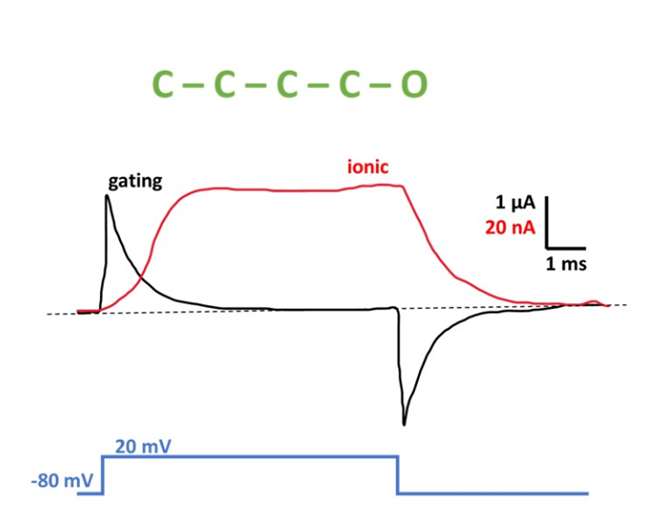
\includegraphics{Picture1.png}

\subsection*{(a) During the activation step, why is gating current transient but ionic current sustained? Why does the gating current appear to peak long before the ionic current?}
\subsection*{(b) At the end of the voltage step, why does the deactivation of the ionic current coincide with the rebound of the gating current (in other words, why is there no delay in this case)?}
\subsection*{(c) A second voltage protocol returns the membrane from +20mV to -40mV rather than -80mV. Using the state model and principles from class, draw the predicted OFF gating current and ionic deactivation current traces relative to the originals. Explain the sign, approximate relative size, and timing of each change.}

\section*{Question 3}
You record the following single channel current trace (idealized) from a typical voltage-gated potassium channel at steady-state in an outside-out patch at +20 mV with equal 150 mM KCl on both sides of the membrane.  Scale bar on the right shows the single channel current amplitude.  Calculate the following. Include relevant equations and correct units.

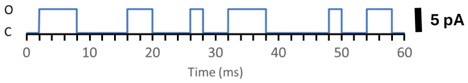
\includegraphics{Picture2.jpg}

\subsection*{(a) Single channel conductance}
\textcolor{blue}{
$$I = \gamma(V_m)$$
$$5\text{pA} = \gamma(20\text{mV})$$
$$\gamma = \frac{5\text{pA}}{20\text{mV}} = \boxed{250\text{pS}}$$
}
\subsection*{(b) Open probability}
\textcolor{blue}{
$$P_{\text{open}} = \frac{t_{\text{open}}}{t_{\text{total}}}$$
$$ = \frac{(6+4+2+6+2+4)\text{ms}}{60\text{ms}} = \frac{24}{60} = \boxed{0.4}$$
}
\subsection*{(c) Mean Open Duration and Mean Closed Duration}
\textcolor{blue}{
$$\mu_{\text{open}} = \frac{t_{\text{open}}}{T_{\text{open}}}$$
where $T_{\text{open}}$ is number of times the channel was open
$$\mu_{\text{open}} = \frac{24\text{ms}}{6} = \boxed{4\text{ms}}$$
}

\textcolor{blue}{
$$\mu_{\text{closed}} = \frac{t_{\text{closed}}}{T_{\text{closed}}}$$
where $T_{\text{closed}}$ is number of times the channel was closed
$$\mu_{\text{closed}} = \frac{(60-24)\text{ms}}{7} = \boxed{5.14\text{ms}}$$
}
\subsection*{(d) Assuming an ideal two-state model (Figure~\ref{fig:two-state}), estimate $\alpha$ and $\beta$ from the dwell intervals and then predict open probability from those rates. How does this prediction compare with your calculation in (b), and explain if they are different?}

\begin{figure}[H]
    \centering
    \caption{Ideal two-state model.}
    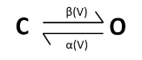
\includegraphics[width=0.3\textwidth]{Picture3.png}
    \label{fig:two-state}
\end{figure}

\textcolor{blue}{
$$\alpha = \frac{1}{\mu_{\text{open}}} = \frac{1}{4\text{ms}} = \boxed{0.25\text{ms}^{-1}}$$
$$\beta = \frac{1}{\mu_{\text{closed}}} = \frac{1}{5.14\text{ms}} = \boxed{0.194\text{ms}^{-1}}$$
}
\textcolor{blue}{
$$\hat{P}_{\text{open}} = \frac{\beta}{\alpha + \beta} = \frac{\frac{7}{36}}{\frac{6}{24}+\frac{7}{36}} = \frac{7}{36} = \boxed{0.4375}$$
}

\textcolor{blue}{
The estimated open probability using $\alpha$ and $\beta$ differs from open probability calculated from $t_{\text{open}}$.
This is likely due to the stochasticity of the system.
If we were to measure the current for longer,
we would see open probability using $\alpha$ and $\beta$ converge to open probability calculated from $t_{\text{open}}$.
}
\section*{Question 4}
You record from a cell heterologously overexpressing a single type of voltage-gated potassium channels (i.e., many channels of a single type are expressed in each cell).  You record under Whole-Cell conditions with normal physiological intracellular and extracellular solutions (namely, Ek=-80) to get the macroscopic steady-state conductance vs voltage curves below under control conditions and in the presence of Drug A and Drug B.  Assume the drugs only effect this potassium channel. Answer the following questions.

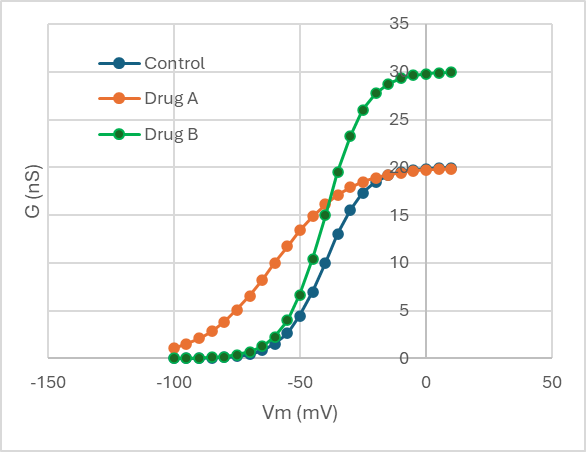
\includegraphics{Picture4.png}

\subsection*{(a) The resting membrane potential for this cell is -60 mV.  How would Drug A change the resting potential (more positive, more negative), if at all?}
\subsection*{(b) How would Drug B change the resting potential, if at all?}
\subsection*{(c) Estimate Vhalf from the curves for control conditions and when exposed to Drug A and Drug B.}
\subsection*{(d) In addition to Vhalf, what parameter in the Boltzmann equation does Drug A appear to impact? Provide at least one hypothesis for how Drug A could affect the voltage sensor S4 to achieve this effect.}
\subsection*{(e) During lab meeting, some argue that Drug B increases channel number, others say it increases single-channel conductance, still others say it increases maximum open probability. State whether the present G-V data can distinguish between these three possibilities.  Briefly, propose one additional experiment that would help discriminate among the viable explanations.}

\end{document}